\documentclass[11pt,a4paper]{article} 
\usepackage{amssymb}
\usepackage[shortlabels]{enumitem}
\usepackage[fleqn]{amsmath} 
\usepackage{relsize}
\usepackage{graphicx}
\usepackage[super]{nth}
\usepackage{hyperref, url}
\usepackage[margin=2cm, top=2cm]{geometry}
\graphicspath{{./img/}}
\newcommand\setItemNumber[1]{\setcounter{enumi}{\numexpr#1-1\relax}}
\newcommand*{\mybox}[1]{\framebox{#1}}
\newcommand{\tuple}[1]{$\langle #1 \rangle$} 
\newcommand{\stuple}[1]{$\langle$#1$\rangle$} % ordered pair with strings inside
\newcommand{\forceindent}{\leavevmode{\parindent=1em\indent}}
\DeclareUnicodeCharacter{2212}{-}
\title{\bf Homework 8\\[1ex]
\rm\normalsize CS250 Discrete Structures I, Winter 2020 }
\date{\normalsize Due: May, 27, 2020}
\author{\normalsize Armant Touche}

\begin{document} 
\vspace{0cm}\maketitle 
	
	
	\subparagraph{Problem 1} 4.1 Graph Definitions (pg. 243-246) \\
			
		From section 4.1 in the textbook, complete exercises 1, 3, 7, 8, 12, 13

        \begin{enumerate}

        %1
        \item  If 10 people each shake hands with each other, how many handshakes took place? What does this question have to do with graph theory?\\
            Using the Handshake Lemma and dividing the sum by two since the sum of degrees counts each edge twice, I am able to compute the number of handshake between 10 people by using
            $$ (\sum_{v\in V} d(10)) = 90\div 2 = 45\;\;\text{(handshakes)}$$

        %3
        \setItemNumber{3}
    \item Is it possible for two \textit{different} (non-isomorphic) graphs to have the same number of vertices and the same number of edges? What if the degrees of the vertices in the two graphs are the same (so both graphs have vertices with degrees 1, 2, 2, 3, and 4, for example)? Draw two such graphs or explain why not.

        %7
        \setItemNumber{7}
        \item Which of the graphs below are bipartite? Justify your answers

            \begin{center}
            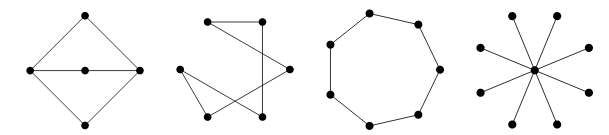
\includegraphics[width=.5\textwidth]{hw8_graphic1}
            \end{center}

        %8
        \item For which $n\geq 3$ is the graph $C_n$ bipartite?\\
            $C_n$ is bipartite such that when $n$ is an even integer.

        %12
        \setItemNumber{12}
    \item We often define graph theory concepts using set theory. For example, given a graph $G = (V, E)$ and a vertex $v\in V$, we define
        $$N(v) = \{u\;\in V\; |\; \{v,u\}\;\in E\}$$
        We define $N[v] = N(v)\cup \{v\}$. The goal of this problem is to figure out what all this means.
        \begin{enumerate}

        \item Let $G$ be the graph with $V = \{a,b,c,d,e,f\}$ and\\ $E = \{\{a,b\},\{a,e\},\{b,c\},\{b,e\},\{c,d\},\{c,f\},\{d,f\},\{e,f\}\}$. \\Find $N(a)$, $N[a]$, $N(c)$, and $N[c]$.\\
            $N(a) = \{ \{a,b\}, \{a,e\}\}\\ N[a] = N(a)\cup \{a\}\\ = \{\emptyset,\{a\},\{a,b\},\{a,e\}\}$\\
            $N(c) = \{\{c,d\},\{c,f\}\}\\N[c] = N(c)\cup\{c\}\\ = \{\emptyset,\{c\}, \{b,c\},\{c,d\},\{c,f\}\}$
        \item What is the largest and smallest possible values for $|N(v)|$ and $|N[v]|$ for the graph in part (a)? Explain.\\
Smallest
        \item Give an example of a graph $G=(V,E)$ (probably different than the one above) for which $N[v]=V$ for some vertex $v\in V$. Is there a graph for which $N[v]=V$ for all $v\in V$? Explain.
        \item Give an example of a graph $G=(V,E)$ for which $N(v)=\emptyset$ for some $v\in V$. Is there an example of such a graph for which $N[u]=V$ for some other $u\in V$ as well? Explain.
        \item Describe in words what $N(v)$ and $N[v]$ mean in general.

        \end{enumerate}

        %13
        \item A graph is a way of representing the relationships between elements in a set: an edge between the vertices $x$ and y tells us that $x$ is related to $y$ (which we can write as $x\sim y$). Not all sorts of relationships can be represented by a graph though. For each relationship described below, either draw the graph or explain why the relationship cannot be represented by a graph.

            \begin{enumerate}
                \item The set $V={1,2,…,9}$ and the relationship $x\sim y$ when $x-y$ is a non-zero multiple of 3.
                \item The set $V={1,2,…,9}$ and the relationship $x\sim y$ when $y$ is a multiple of $x$.
                \item The set $V={1,2,…,9}$ and the relationship $x\sim y$ when $0<|x−y|<3$.

            \end{enumerate}
        \end{enumerate}
	
	\subparagraph{Problem 2} 4.2 Proofs (pg. 255-257) \\
	
		From section 4.2 in the textbook, complete exercises 2, 3, 4, 7, 11, 13

        \begin{enumerate}

        %2
        \setItemNumber{2}
        \item For each degree sequence below, decide whether it must always, must never, or could possibly be a degree sequence for a tree. Remember, a degree sequence lists out the degrees (number of edges incident to the vertex) of all the vertices in a graph in non-increasing order.

            \begin{enumerate}
                \item (4,1,1,1,1)
                \item (3,3,2,1,1)
                \item (2,2,2,1,1)
                \item (4,4,3,3,3,2,2,1,1,1,1,1,1,1)

            \end{enumerate}

        %3
        \item For each degree sequence below, decide whether it must always, must never, or could possibly be a degree sequence for a tree. Justify your answers.

            \begin{enumerate}
                \item (3,3,2,2,2)
                \item (3,2,2,1,1,1)
                \item (3,3,3,1,1,1)
                \item (4,4,1,1,1,1,1,1)
            \end{enumerate}

        %4
        \item Suppose you have a graph with $v$ vertices and $e$ edges that satisfies $v=e+1$. Must the graph be a tree? Prove your answer.

        %7
        \setItemNumber{7}
        \item We define a \textbf{\emph{forest}} to be a graph with no cycles.
            \begin{enumerate}
                \item Explain why this is a good name. That is, explain why a forest is a union of trees.
                \item Suppose $F$ is a forest consisting of $m$ trees and $v$ vertices. How many edges does $F$ have? Explain.
                \item Prove that any graph $G$ with $v$ vertices and $e$ edges that satisfies $v<e+1$ must contain a cycle (i.e., not be a forest).
            \end{enumerate}

        %11
        \setItemNumber{11}
        \item Let $T$ be a rooted tree that contains vertices $u$, $v$, and $w$ (among possibly others). Prove that if $w$ is a descendant of both $u$ and $v$, then $u$ is a descendant of $v$ or $v$ is a descendant of $u$.

        \setItemNumber{13} Find all spanning trees of the graph below. How many different spanning trees are there? How many different spanning trees are there up to isomorphism (that is, if you grouped all the spanning trees by which are isomorphic, how many groups would you have)?

            \begin{center}
            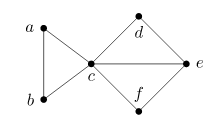
\includegraphics[width=.45\textwidth]{hw8_graphic2}
            \end{center}

        \end{enumerate}
	
	
	
		
\end{document}
